Веб-сайт представляет собой набор связанных веб-страниц, включая мультимедийный контент, обычно идентифицированный с общим доменным именем, и опубликованный на
по крайней мере, один веб-сервер. Известными примерами являются wikipedia.org, google.com и amazon.com.

Веб-сайт может быть доступен через общедоступную сеть Интернет-про-токола (IP), такую как Интернет или частную локальную сеть (LAN), путем ссылки на
единый локатор ресурсов (URL), который идентифицирует сайт.

Веб-сайты могут иметь много функций и могут использоваться в различных моделях; веб-сайт может быть личным веб-сайтом, корпоративным веб-сайтом для компании, правительственным
веб-сайтом, веб-сайтом организации и т. д. Веб-сайты, как правило, предназначены для определенной темы или цели, начиная от развлечений и социальных сетей
заканчивая новостями и образовательными сайтами. Все общедоступные веб-сайты в совокупности составляют Всемирную паутину, а частные веб-сайты, такие как
сайт для сотрудников, как правило, являются частью интрасети.

По технологическим особенностям сайты различаются:

\begin{itemize}
\item Статические -- состоящие из статичных html (htm, dhtml) страниц, составляющих единое целое. Пользователю выдаются файлы в том виде, в котором они хранятся на сервере.
\item Динамические -- состоящие из динамичных html (htm, dhtml) страниц-шаблонов, информации, скриптов и прочего в виде отдельных файлов. Содержимое генерируется по запросу
специальными скриптами (программами) на основе других данных из любого источника
\item Одностраничные приложения -- тип полностью динамических веб приложений, при котором все приложение располагается на единой веб-странице и доступ к частям приложения
осуществляется посредством динамической догрузки данных в процессе использования. Такие приложения, как правило, используется в тандеме с RESTful веб-сервисом и реализуют
большую долю своей логики на стороне клиента (с помощью Javascript).
\item Сайты, созданные с применением т. н. Flash-технологий, когда весь сайт располагается на одной веб-странице, предназначенной исключительно для загрузки Flash-файла,
а вся навигация и контент реализованы в самом Flash-ролике. Являются частным случаем одностраничных приложений.
\end{itemize}

По типам макетов, используемых при разработке:
\begin{itemize}
\item Фиксированной ширины (англ. rigid fixed) -- размеры элементов страницы имеют фиксированное значение, независящее от разрешения, размера, соотношения сторон экрана
монитора и размеров окна обозревателя, задаётся в абсолютных значениях -- PX (пиксели).
\item Резиновый макет (англ. adaptable fluid) -- размеры несущих элементов, значения ширины, задаются относительным значением -- процентами,
страницы отображаются во весь экран монитора по ширине.
\item Динамично эластичный (англ. dynamically expandable elastic) -- размеры большинства элементов задаются относительными значениями -- EM
и процентами. Все относительные пропорции размеров элементов всегда остаются неизменными, независимо от разрешения, размера, соотношения
сторон экрана монитора, размеров окна и масштаба окна обозревателя. И всегда постоянны относительно окна обозревателя.
\end{itemize}

\subsubsection{Одностраничные веб-приложения}
\label{sub:domain:overview_website:spa}
Одностраничное приложение (англ. single page application, SPA) -- это веб-приложение или веб-сайт, использующий единственный HTML-документ как оболочку для всех веб-страниц 
и организующий взаимодействие с пользователем через динамически подгружаемые HTML, CSS, JavaScript, обычно посредством AJAX. Приложение такого типа появились 
сравнительно недавно, с началом эры HTML5 и SPA является типичным представителем приложений на HTML5. SPA напоминают родные (native) приложения, с той лишь разницей, 
что исполняются в рамках браузера, а не в собственном процессе операционной системы.

Одностраничные приложения работают в рамках браузера и не требуют перезагрузки страницы или загрузки дополнительных страниц во время использования. Подобные 
приложения ежедневно используют миллионы юзеров, даже не замечая этого. Самые популярные примеры:  GitHub, Gmail, Google Maps и даже Facebook. Одностраничные приложения, 
как правило, максимально интерактивны, причём настолько, что у пользователя складывается ощущение, будто он работает с десктопным приложением: реакция приложения 
на пользовательские действия моментальная в большинстве случаев. Этим SPA выгодно отличаются от многостраничных сайтов, где при каждом действии пользователю необходимо 
дожидаться загрузки новой страницы.

SPA запрашивает разметку страницы и её контент, а затем создает конечный вид страницы непосредственно в браузере. Такого эффекта можно достигнуть благодаря продвинутым
фреймворкам JavaScript, таким как AngularJS, Ember.js, Meteor.js, Knockout.js.

\begin{figure}[ht]
\centering
  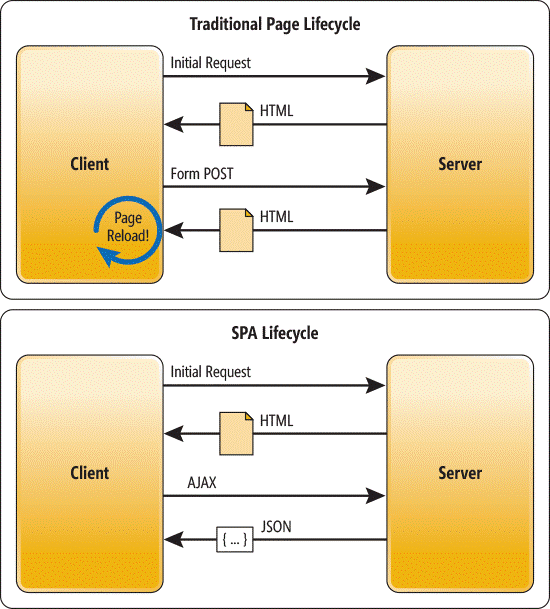
\includegraphics[scale=0.75]{spa.png}
  \caption{Жизненный цикл одностраничного приложения в сравнении с традиционным подходом}
  \label{figure:domain:spa}
\end{figure}

Преимущества одностраничных приложений:
\begin{itemize}
\item SPA характеризуются отличным быстродействием, так как большинство ресурсов, которые они используют (HTML+CSS+Скрипты), загружаются лишь однажды в течение сессии 
использования приложения. После совершения действий на странице меняются лишь данные.
\item Разработка веб-приложений обычно быстрее и эффективнее. Нет необходимости писать отдельный код для рендера страницы на стороне сервера. Также гораздо легче 
запустить процесс разработки подобных приложений, потому что писать код можно начинать с файла file://URI, не используя при этом никакой сервер.
\item SPA оптимизированы для Chrome debugging, разработчики могут отслеживать сетевые действия, изучать элементы страниц и данные, с ними ассоциируемые.
\item Если у вас уже есть SPA, будет возможность с тем же бэкендом создать и мобильное приложение.
\item SPA более эффективны в кэшировании данных на локальных носителях. Приложение высылает один запрос, собирает все необходимые данные, и с этого момента
 способно работать даже в режиме оффлайн.
\end{itemize}

Недостатки одностраничных приложений:
\begin{itemize}
\item SEO-оптимизация одностраничных приложений, по очевидным причинам, не очень проста. Контент приложений загружается при помощи AJAX (A-synchronous JavaScript and XML) -- метода
 обмена данными и обновления приложения без перезагрузки страницы, в то время как SEO-оптимизация основана на устойчивости контента в каждой отдельно взятой странице. При этом 
 продвижение вашего сайта в поисковиках не невозможно. Многие изменения в SEO можно провести на стороне сервера, а компании вроде Google продолжают придумывать новые решения для
 того, чтобы облегчить жизнь как владельцам SPA, так и их пользователям.
\item Они достаточно долго загружаются, поскольку тяжелые клиентские фреймворки должны сперва загрузиться в браузер.
\item SPA требуют JavaScript в активном режиме в браузерах пользователей. Если кто-то из ваших клиентов вручную отключит использование JavaScript, они не смогут в полной мере
воспользоваться вашим приложением. Даже если вы будете кэшировать и обрабатывать ваши страницы на стороне сервера (а это сейчас тоже возможно), вы всё ещё рискуете не доставить 
пользователям без JS все функции одностраничного приложения в правильном виде.
\item По сравнению с традиционными приложениями, SPA чуть хуже защищены. Благодаря межсайтовому скриптингу (XSS), злоумышленники имеют возможность внедрять дополнительные 
скрипты на стороне клиента.
\item Некоторые утечки памяти в JavaScript могут привести к падению производительности даже в мощных системах
 \end{itemize}

Исходя из вышеперечисленных преимущств и недостатков, можно заключить что SPA подходят для реализации приложений для редактирования некоторого пользовательского содержимого,
например для создания приложения для редактирования трехмерных моделей. Продолжительная работа с таким приложением не будет затруднена постоянными перезагрузками страниц, а
инкрементальное сохранение прогресса пользователя может быть реализовано в фоновом процессе.
